\chapter{Multivariate Linear Regression and Inference}
\label{ch:regression-multi}

\begin{chaptergoals}
\begin{itemize}[nosep]
\item Several predictors at once: the model $Y = X\beta + \epsilon$ with a design matrix $X$, which also covers polynomials, $0/1$ variables and the previous eruption's wait and duration for Old Faithful.
\item Least squares in matrix form, $\hat{\beta} = (X^\top X)^{-1}X^\top Y$, and what it is: the projection of the response vector onto the space spanned by the columns of $X$. Full rank as identifiability.
\item With Gaussian errors: the distribution of $\hat{\beta}$, the residual variance on $n - p$ degrees of freedom by the general form of Cochran's theorem, the exact $t$-test for one coefficient and the $F$-test for several, which is the likelihood ratio test. Bonferroni as the alternative.
\item Why a coefficient depends on which other predictors are in the model, and why two predictors can matter together when neither does alone.
\item Ridge in matrix form, large samples without Gaussian errors, and what a fitted model does and does not show.
\end{itemize}
\Cref{ch:regression-uni} fit one line; this chapter fits a plane, or a hyperplane, with the same arithmetic written in matrices, and the exact $t$ of that chapter becomes a $t$ and an $F$.
\end{chaptergoals}

\section{Several predictors at once}
\label{sec:mreg-model}

Chapter \ref{ch:regression-uni} ended with the remark that Old Faithful's next wait might depend not only on the eruption just ended but on the eruption before it.
Most responses are like that.
The example that runs through this chapter is older and smaller.
A plant oxidizes ammonia to nitric acid, and some of the ammonia escapes up the stack unconverted.
Brownlee (\textit{Statistical Theory and Methodology in Science and Engineering}, 1965) reported, for $21$ days of operation, the stack loss, ten times the percentage of ammonia lost, together with three things the operators could watch: the air flow into the plant, the temperature of the cooling water, and the concentration of the circulating acid (coded, so that $89$ means $58.9\%$).
The data are in the table, and \cref{fig:mregpredictors} plots the loss against each of the three; the question is how the loss depends on the three together.

\begin{center}
\small
\setlength{\tabcolsep}{3.1pt}
\begin{tabular}{@{}lrrrrrrrrrrrrrrrrrrrrr@{}}
\toprule
day & 1 & 2 & 3 & 4 & 5 & 6 & 7 & 8 & 9 & 10 & 11 & 12 & 13 & 14 & 15 & 16 & 17 & 18 & 19 & 20 & 21 \\
\midrule
air flow & 80 & 80 & 75 & 62 & 62 & 62 & 62 & 62 & 58 & 58 & 58 & 58 & 58 & 58 & 50 & 50 & 50 & 50 & 50 & 56 & 70 \\
water temperature & 27 & 27 & 25 & 24 & 22 & 23 & 24 & 24 & 23 & 18 & 18 & 17 & 18 & 19 & 18 & 18 & 19 & 19 & 20 & 20 & 20 \\
acid concentration & 89 & 88 & 90 & 87 & 87 & 87 & 93 & 93 & 87 & 80 & 89 & 88 & 82 & 93 & 89 & 86 & 72 & 79 & 80 & 82 & 91 \\
stack loss & 42 & 37 & 37 & 28 & 18 & 18 & 19 & 20 & 15 & 14 & 14 & 13 & 11 & 12 & 8 & 7 & 8 & 8 & 9 & 15 & 15 \\
\bottomrule
\end{tabular}
\end{center}

\begin{figure}[htbp]
\centering
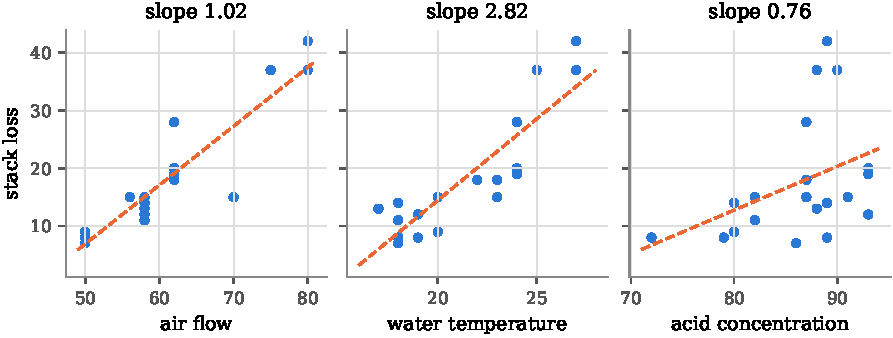
\includegraphics[width=\textwidth]{fig_mreg_predictors}
\caption{The stack loss data, $21$ days: the loss against the air flow, the cooling water temperature and the acid concentration, each with the least squares line of the loss on that predictor alone (orange, dashed).}
\label{fig:mregpredictors}
\end{figure}

With one predictor the model was $Y_i = a + bx_i + \epsilon_i$.
With three it is $Y_i = \beta_1 + \beta_2 x_{i2} + \beta_3 x_{i3} + \beta_4 x_{i4} + \epsilon_i$, and the natural way to write $n$ such equations is as one equation between vectors.

\begin{definition}[Linear regression model with several predictors]
\label{def:mreg-model}
Let $X$ be an $n \times p$ matrix of fixed numbers, the \textbf{design matrix}, whose row $i$ is $x_i^\top = (x_{i1}, \ldots, x_{ip})$, the $p$ predictor values of observation $i$; usually $x_{i1} = 1$ for every $i$, so that $\beta_1$ is the intercept.
The \textbf{linear regression model} says
\[
Y = X\beta + \epsilon, \qquad \text{that is,} \qquad Y_i = x_i^\top\beta + \epsilon_i, \quad i = 1, \ldots, n,
\]
for an unknown $\beta \in \real^p$, where $Y = (Y_1, \ldots, Y_n)^\top$ and the errors $\epsilon = (\epsilon_1, \ldots, \epsilon_n)^\top$ have mean $0$, a common variance $\sigma^2$ and no correlation: $\E[\epsilon] = 0$ and $\cov(\epsilon) = \sigma^2 I_n$.
The \textbf{Gaussian linear model} assumes moreover $\epsilon \sim \Gauss_n(0, \sigma^2 I_n)$, that is, $\epsilon_1, \ldots, \epsilon_n \iid \Gauss(0, \sigma^2)$.
\end{definition}

\begin{inwords}
Each response is a weighted sum of its predictor values, with the same weights $\beta$ for every observation, plus an error that behaves like every other error. The design matrix holds the data on the predictors, one row per observation and one column per predictor, and $X\beta$ is the vector of the $n$ means $\E[Y_i]$. The model of \cref{ch:regression-uni} is the case $p = 2$, with columns $(1, \ldots, 1)^\top$ and $(x_1, \ldots, x_n)^\top$ and $\beta = (a, b)^\top$.

\textbf{For the kiss data.} With no predictor the design matrix is the single column $(1, \ldots, 1)^\top$, $p = 1$, and $Y = X\beta + \epsilon$ says $R_i = p + \epsilon_i$: every couple has the same mean. A design with two columns, a column of ones and a column of $0$s and $1$s marking the couples observed in one of two cities, say, would let the mean differ between the cities, as the aspirin design of \cref{ex:reg-aspirin} let the heart-attack rate differ between the groups.
\end{inwords}

For the stack loss data, $n = 21$, $p = 4$, and row $1$ of $X$ is $(1, 80, 27, 89)$.
The model is linear in $\beta$, not necessarily in the measured variables, which is what makes it so general.
For Old Faithful, a design with columns $1$, $x_i$ and $x_i^2$ fits a parabola to the waits, and $x_i^2$ is simply a third column of numbers; a design with columns $1$, the duration and the previous wait lets the previous wait in; and a column of $0$s and $1$s, like the aspirin column of \cref{ex:reg-aspirin}, lets two groups have different means.
Treating the $x_i$ as fixed, and reading observational data through the conditional distribution of $Y$ given $X$, is as in \cref{sec:reg-model}.

\begin{remark}[The random-design version]
\Cref{ch:models} wrote the regression model with rows $x_i$ drawn from $\Gauss_d(0, I_d)$ and errors of variance $1$, as an example of a parametric model with $\Theta = \real^d$.
Condition on the drawn rows and that model is the Gaussian linear model of this chapter with $\sigma^2 = 1$ known; this chapter's $\Theta = \real^p \times (0, \infty)$ adds the unknown variance.
Every level and coverage statement below holds given the rows, and so, by the tower-property argument of \cref{sec:reg-model}, unconditionally as well; the distributions and moments themselves, such as $\cov(\hat{\beta}) = \sigma^2(X^\top X)^{-1}$, are statements given the rows.
\end{remark}

\section{Least squares in matrix form}
\label{sec:mreg-lse}

With one predictor, least squares minimized a sum of squared vertical distances.
In vector form that sum is the squared length of $Y - X\beta$, and minimizing a length is a problem in geometry.

\begin{definition}[Least squares estimator]
\label{def:mreg-lse}
The \textbf{least squares estimator} $\hat{\beta}$ minimizes the sum of squared errors
\[
\norm{Y - X\beta}^2 = \sum_{i=1}^n (Y_i - x_i^\top\beta)^2
\]
over $\beta \in \real^p$; the \textbf{fitted values} are $\hat{Y} = X\hat{\beta}$ and the \textbf{residuals} are $e = Y - \hat{Y}$.
\end{definition}

\begin{inwords}
Least squares picks, among all vectors of the form $X\beta$ (the column space of $X$ \toolkit{sec:math-matrices}), the one closest to the response vector $Y$ in ordinary Euclidean distance. The residuals are what is left over, observation by observation.

\textbf{For the kiss data.} With the single column of ones, $\norm{Y - X\beta}^2 = \sum_i (R_i - \beta)^2$ is smallest at $\beta = \bar{R}_n = 0.645$; the fitted vector is $0.645$ in every coordinate and the residuals are $0.355$ and $-0.645$ as in \cref{ch:regression-uni}.
\end{inwords}

The one-predictor theorem of \cref{ch:regression-uni} needed the $x_i$ not to be all equal.
The general condition is that the columns of $X$ be linearly independent: no column is a combination of the others, so that $X\beta = X\beta'$ only when $\beta = \beta'$, which is the statement that $X$ has rank $p$ \toolkit{sec:math-matrices}.

\begin{theorem}[The least squares estimator and the projection]
\label{thm:mreg-lse}
If $X$ has rank $p$, then $X^\top X$ is invertible and the least squares estimator is unique,
\[
\hat{\beta} = (X^\top X)^{-1}X^\top Y.
\]
The fitted vector is $\hat{Y} = PY$, with $P = X(X^\top X)^{-1}X^\top$ the matrix of the orthogonal projection onto the column space of $X$, and the residual vector $e = (I - P)Y$ is perpendicular to every column of $X$: $X^\top e = 0$.
\end{theorem}
\coreproof{The closest point to $Y$ in a subspace is the foot of the perpendicular, and the residual is perpendicular to the subspace. Perpendicular to every column means $X^\top(Y - X\hat{\beta}) = 0$, which are $p$ linear equations in $\hat{\beta}$ with the invertible matrix $X^\top X$.}
\begin{proof}
If $X^\top Xa = 0$ then $a^\top X^\top Xa = \norm{Xa}^2 = 0$, so $Xa = 0$ and, the columns being independent, $a = 0$: $X^\top X$ is invertible.
Let $\hat{\beta} = (X^\top X)^{-1}X^\top Y$ and $e = Y - X\hat{\beta}$.
Then $X^\top e = X^\top Y - X^\top X(X^\top X)^{-1}X^\top Y = 0$: the residual is perpendicular to the columns of $X$, hence to every vector $Xb$ in the column space.
For any $\beta$, write $Y - X\beta = e + X(\hat{\beta} - \beta)$, a sum of two perpendicular vectors, so by Pythagoras
\[
\norm{Y - X\beta}^2 = \norm{e}^2 + \norm{X(\hat{\beta} - \beta)}^2 \geq \norm{e}^2,
\]
with equality only when $X(\hat{\beta} - \beta) = 0$, that is, $\beta = \hat{\beta}$.
So $\hat{\beta}$ is the unique minimizer.
The matrix $P$ satisfies $P^\top = P$ and $P^2 = X(X^\top X)^{-1}X^\top X(X^\top X)^{-1}X^\top = P$, it fixes every vector in the column space ($PXb = Xb$) and sends every vector perpendicular to the columns to $0$, which is what the orthogonal projection does \toolkit{sec:math-matrices}; and $X\hat{\beta} = PY$ by the formula for $\hat{\beta}$.
\end{proof}

\Cref{fig:mregprojection} draws the theorem: the column space of $X$ as a plane through the origin, the response $Y$ as a vector above it, the fitted vector as the foot of the perpendicular from $Y$ to the plane, and the residual as the perpendicular itself.
Least squares is nothing but this picture, in $n$ dimensions.
The $p$ equations $X^\top e = 0$ are the \textbf{normal equations}; for the design with a column of ones and one predictor they are the two of \cref{thm:lse}, $\sum_i e_i = 0$ and $\sum_i x_ie_i = 0$.

\begin{figure}[htbp]
\centering
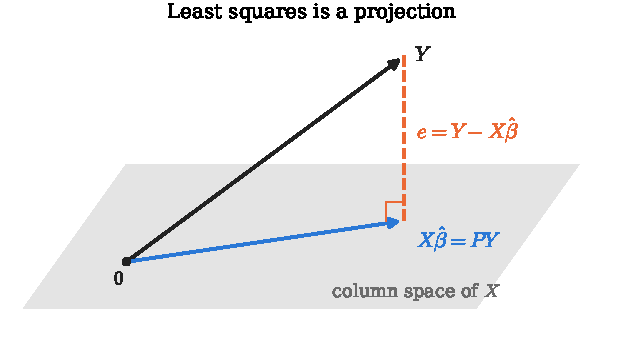
\includegraphics[width=0.62\textwidth]{fig_mreg_projection}
\caption{Least squares as a projection: the column space of $X$ (gray), the response vector $Y$ (black), the fitted vector $X\hat{\beta}$ (blue), the foot of the perpendicular from $Y$, and the residual $e$ (orange, dashed).}
\label{fig:mregprojection}
\end{figure}

\begin{worked}[the stack loss fit]
For the $21$ days, solving the normal equations gives
\[
\hat{\beta} = (-39.92,\ 0.716,\ 1.295,\ -0.152)^\top:
\]
in words, with the air flow, the water temperature and the acid concentration,
\[
\text{predicted loss} = -39.92 + 0.716\,(\text{air}) + 1.295\,(\text{water}) - 0.152\,(\text{acid}).
\]
Each unit of air flow adds $0.72$ to the loss when the other two are held fixed, each degree of water temperature adds $1.3$, and each unit of acid concentration subtracts $0.15$. The residual sum of squares is $\norm{e}^2 = 178.8$, against $\sum_i (Y_i - \bar{Y})^2 = 2{,}069.2$ for the constant fit, so the three predictors account for $1 - 178.8/2{,}069.2 = 91\%$ of the variation in the loss. \Cref{fig:mregstackloss} plots the observed losses against the fitted ones and the residuals against the fitted values; day $21$, with air flow $70$ and a loss of only $15$, is the worst-fitted day, with residual $-7.2$.
\end{worked}

\begin{figure}[htbp]
\centering
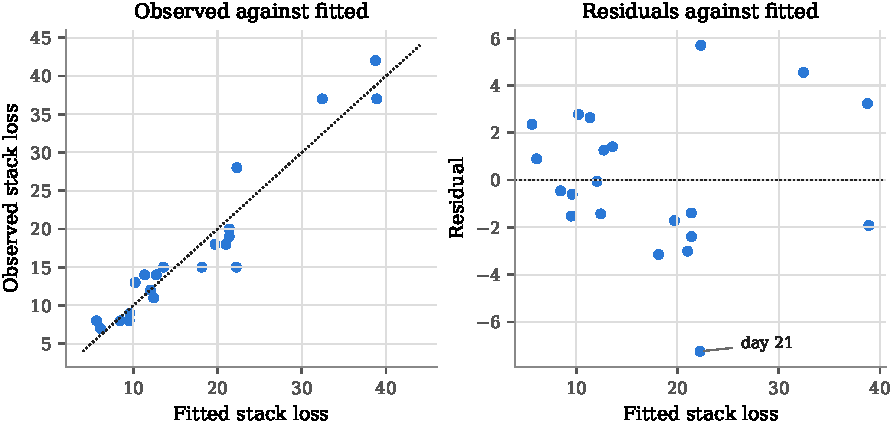
\includegraphics[width=\textwidth]{fig_mreg_stackloss}
\caption{The stack loss fit. Left: observed stack loss against the fitted values of the three-predictor model, with the line $y = x$ (dotted). Right: the residuals against the fitted values; day $21$ is the lowest point.}
\label{fig:mregstackloss}
\end{figure}

The coefficient $0.716$ is not the slope of the loss on the air flow alone, which \cref{fig:mregpredictors} drew, and the difference is the first thing to understand about a multiple regression.

\begin{sanitycheck}[A coefficient on its own, and in company]
Regress the loss on the air flow alone and the slope is $1.02$, not $0.72$. Both are right: $1.02$ is the change in loss per unit of air flow when the water temperature and the acid are left to vary as they did, and on these days warmer water went with higher air flow (correlation $0.78$), so the air flow alone gets credit for the water's effect as well. The multiple regression coefficient $0.72$ is the change per unit of air flow with the other two held fixed.
\end{sanitycheck}

When the columns of $X$ are dependent, the least squares problem still has a solution, the projection $PY$ onto the column space, but infinitely many $\beta$ produce it.

\needspace{12\baselineskip}
\begin{pitfall}[collinearity is non-identifiability]
If one column is a combination of the others, say $x_{i3} = 2x_{i2}$ for every $i$, then $X\beta = X\beta'$ whenever $\beta'$ moves weight from $\beta_2$ to $\beta_3$ in the ratio $2 : 1$. The distribution of $Y$ depends on $\beta$ only through $X\beta$, so two different parameters give the same distribution: the parameter is not identifiable, in the sense of \cref{ch:models}, and no data can tell $\beta$ from $\beta'$. Software reports it by dropping a column. A milder form appears when the columns are nearly dependent (\cref{sec:mreg-ttest}): $\hat{\beta}$ exists but has a large variance in the direction where the columns almost cancel.
\end{pitfall}

\section{The Gaussian linear model}
\label{sec:mreg-gaussian}

Everything \cref{ch:regression-uni} proved for one predictor holds for $p$, with $(X^\top X)^{-1}$ where $1/S_{xx}$ was.
The tool is the general form of Cochran's theorem, promised in \cref{ch:t-test}.

\begin{proposition}[Cochran's theorem, general form]
\label{prop:cochran-general}
Let $\epsilon \sim \Gauss_n(0, \sigma^2I_n)$, and let $\real^n$ be split into mutually perpendicular subspaces $S_1, \ldots, S_m$ of dimensions $d_1 + \cdots + d_m = n$, with orthogonal projections $P_1, \ldots, P_m$.
Then $\norm{P_1\epsilon}^2/\sigma^2, \ldots, \norm{P_m\epsilon}^2/\sigma^2$ are independent, with $\norm{P_j\epsilon}^2/\sigma^2 \sim \chi^2_{d_j}$.
\end{proposition}
\coreproof{Rotate to an orthonormal basis adapted to the subspaces, $d_1$ vectors spanning $S_1$, then $d_2$ spanning $S_2$, and so on. The rotated coordinates are independent $\Gauss(0, \sigma^2)$, and each $\norm{P_j\epsilon}^2$ is the sum of the squares of its own block of them.}
\begin{proof}
Choose an orthonormal basis of each $S_j$ and put them together: since the subspaces are perpendicular and their dimensions add to $n$, these are $n$ orthonormal vectors, and orthonormal vectors are linearly independent (dotting $\sum_k c_ku_k = 0$ with $u_j$ gives $c_j = 0$), so they are an orthonormal basis $u_1, \ldots, u_n$ of $\real^n$.
Let $Q$ be the orthogonal matrix with rows $u_k^\top$ and $Z = Q\epsilon$, so $Z_k = u_k^\top\epsilon$ and $\epsilon = \sum_k Z_ku_k$; by rotation invariance \toolkit{sec:math-gaussvec}, $Z_1, \ldots, Z_n$ are i.i.d.\ $\Gauss(0, \sigma^2)$.
The projection $P_j$ keeps the terms of $\sum_k Z_ku_k$ whose $u_k$ lie in $S_j$ and kills the rest, so $\norm{P_j\epsilon}^2$ is the sum of $Z_k^2$ over the $d_j$ indices of that block.
The blocks are disjoint, so the $m$ sums are independent, and each divided by $\sigma^2$ is a sum of $d_j$ squared independent standard Gaussians.
\end{proof}

\Cref{thm:cochran} is the case $m = 2$ with $S_1$ the line through $(1, \ldots, 1)$; the proofs below use $m = 2$ and $m = 3$ with the column space of $X$ in place of the line.

\begin{theorem}[Least squares with $p$ predictors]
\label{thm:mreg-exact}
In the linear regression model with $X$ of rank $p$ and $n > p$:
\begin{enumerate}[nosep]
\item $\E[\hat{\beta}] = \beta$ and $\cov(\hat{\beta}) = \sigma^2(X^\top X)^{-1}$, so the quadratic risk is $\E\norm{\hat{\beta} - \beta}^2 = \sigma^2\,\mathrm{tr}\big((X^\top X)^{-1}\big)$;
\item $\E\norm{e}^2 = (n - p)\sigma^2$, so $\hat{\sigma}^2 = \norm{e}^2/(n - p)$ is an unbiased estimator of $\sigma^2$.
\end{enumerate}
In the Gaussian linear model, moreover:
\begin{enumerate}[nosep]
\setcounter{enumi}{2}
\item $\hat{\beta} \sim \Gauss_p\big(\beta, \sigma^2(X^\top X)^{-1}\big)$, and the maximum likelihood estimators are $\hat{\beta}$ and $\norm{e}^2/n$;
\item $(n - p)\hat{\sigma}^2/\sigma^2 \sim \chi^2_{n-p}$, independent of $\hat{\beta}$;
\item for each $j$, with $\gamma_j$ the $j$th diagonal entry of $(X^\top X)^{-1}$,
\[
\frac{\hat{\beta}_j - \beta_j}{\hat{\sigma}\sqrt{\gamma_j}} \sim t_{n-p}.
\]
\end{enumerate}
\end{theorem}
\coreproof{$\hat{\beta} - \beta$ is a fixed matrix times the error vector, which gives the mean and covariance at once. For the residuals, rotate the errors so that the first $p$ axes span the column space: the fit absorbs those $p$ coordinates and the residual is the other $n - p$, which is \cref{prop:cochran-general} with the column space and its orthogonal complement.}
\recall{The chi-squared distribution (\cref{def:chisq}): a sum of $k$ squared independent standard Gaussians is $\chi^2_k$. Student's distribution (\cref{def:student}): if $Z \sim \Gauss(0, 1)$ and $V \sim \chi^2_k$ are independent, $Z/\sqrt{V/k} \sim t_k$. A Gaussian vector (\cref{sec:math-gaussquad}): if $W \sim \Gauss_n(0, \sigma^2 I_n)$ and $B$ is a $p \times n$ matrix of rank $p$, then $BW \sim \Gauss_p(0, \sigma^2 BB^\top)$.}
\begin{proof}
Substituting $Y = X\beta + \epsilon$ into the formula for $\hat{\beta}$,
\[
\hat{\beta} = (X^\top X)^{-1}X^\top(X\beta + \epsilon) = \beta + B\epsilon, \qquad B = (X^\top X)^{-1}X^\top,
\]
so $\E[\hat{\beta}] = \beta$ and $\cov(\hat{\beta}) = B\,\cov(\epsilon)\,B^\top = \sigma^2(X^\top X)^{-1}X^\top X(X^\top X)^{-1} = \sigma^2(X^\top X)^{-1}$ \toolkit{sec:math-gaussquad}.
The risk is $\E\norm{\hat{\beta} - \beta}^2 = \sum_j \var(\hat{\beta}_j)$, the sum of the diagonal entries of the covariance matrix, which is (1).

For (2), rotate.
By Gram--Schmidt \toolkit{sec:math-gaussvec} there is an orthonormal basis $u_1, \ldots, u_n$ of $\real^n$ whose first $p$ vectors span the column space of $X$; let $Q$ be the orthogonal matrix with rows $u_k^\top$ and set $Z = Q\epsilon$, so $Z_k = u_k^\top\epsilon$ and $\epsilon = \sum_k Z_ku_k$.
The $Z_k$ have mean $0$, variance $\sigma^2$ and are uncorrelated, since $\E[Z_jZ_k] = u_j^\top\cov(\epsilon)u_k = \sigma^2u_j^\top u_k$.
The projection $P$ fixes $u_1, \ldots, u_p$ and kills $u_{p+1}, \ldots, u_n$, so
\[
e = (I - P)Y = (I - P)(X\beta + \epsilon) = (I - P)\epsilon = \sum_{k=p+1}^n Z_ku_k, \qquad \norm{e}^2 = Z_{p+1}^2 + \cdots + Z_n^2,
\]
whose mean is $(n - p)\sigma^2$.
Likewise $\hat{\beta} - \beta = B\epsilon = B\sum_{k \leq p} Z_ku_k$, since $Bu_k = (X^\top X)^{-1}X^\top u_k = 0$ for $k > p$ ($u_k$ is perpendicular to the columns): $\hat{\beta}$ is a function of $Z_1, \ldots, Z_p$ alone.

With Gaussian errors, $Z/\sigma = Q(\epsilon/\sigma)$ has i.i.d.\ $\Gauss(0, 1)$ coordinates by rotation invariance \toolkit{sec:math-gaussvec}.
Then $\hat{\beta} = \beta + B\epsilon$ is Gaussian with the covariance of (1), since $B$ has rank $p$ (its $p$ rows are independent because $BX = I_p$); the log-likelihood is $-\frac{n}{2}\log(2\pi\sigma^2) - \norm{Y - X\beta}^2/(2\sigma^2)$, largest in $\beta$ where the sum of squares is smallest, so the maximum likelihood estimator of $\beta$ is $\hat{\beta}$, and then, as in \cref{prop:lse-mle}, its derivative in $\sigma^2$ at $\hat{\beta}$ is $-n/(2\sigma^2) + \norm{e}^2/(2\sigma^4)$, zero at $\sigma^2 = \norm{e}^2/n$: this is (3).
$(n - p)\hat{\sigma}^2/\sigma^2 = \sum_{k > p}(Z_k/\sigma)^2$ is $\chi^2_{n-p}$ by \cref{prop:cochran-general} with $S_1$ the column space and $S_2$ its orthogonal complement, and it is a function of $Z_{p+1}, \ldots, Z_n$ while $\hat{\beta}$ is a function of $Z_1, \ldots, Z_p$, so the two are independent: this is (4).
Finally $(\hat{\beta}_j - \beta_j)/(\sigma\sqrt{\gamma_j})$ is a standard Gaussian, independent of the $\chi^2_{n-p}$ variable of (4); dividing by $\sqrt{\hat{\sigma}^2/\sigma^2}$ gives $t_{n-p}$, which is (5).
\end{proof}

The fit takes $p$ dimensions and the residual the other $n - p$, which is why the divisor is $n - p$: $n - 1$ for a mean, $n - 2$ for a line, $17$ for the stack loss fit.

\begin{worked}[standard errors for the stack loss coefficients]
$\hat{\sigma} = \sqrt{178.8/17} = 3.24$, and the diagonal of $(X^\top X)^{-1}$ is $(13.45, 0.00173, 0.0129, 0.00232)$, so the standard errors $\hat{\sigma}\sqrt{\gamma_j}$ are $11.9$, $0.135$, $0.368$ and $0.156$. The $95\%$ confidence interval for the air flow coefficient is $0.716 \pm 2.110 \times 0.135 = [0.43, 1.00]$, with $q_{0.025}(t_{17}) = 2.110$; for the water temperature, $[0.52, 2.07]$; for the acid, $[-0.48, 0.18]$, which contains $0$. The quadratic risk of $\hat{\beta}$ is $\sigma^2 \times 13.47$, almost all of it from the intercept, whose variance is large because the predictors are far from $0$: air flow averages $60$, so the height of the fitted plane at air flow $0$ is an extrapolation.
\end{worked}

\section{One coefficient at a time}
\label{sec:mreg-ttest}

Part (5) of \cref{thm:mreg-exact} gives the test of \cref{ch:regression-uni} for every coefficient.
In the Gaussian linear model, the test of $H_0: \beta_j = 0$ against $H_1: \beta_j \neq 0$ that rejects when
\[
\abs{T_j} > q_{\alpha/2}(t_{n-p}), \qquad T_j = \frac{\hat{\beta}_j}{\hat{\sigma}\sqrt{\gamma_j}},
\]
has level exactly $\alpha$.
Its null hypothesis says that predictor $j$ adds nothing to a model that already contains the other $p - 1$.

\begin{worked}[which predictors matter for the stack loss]
$T = 5.31$ for the air flow and $3.52$ for the water temperature, both beyond $2.110$, with $p$-values $0.0001$ and $0.003$; $T = -0.97$ for the acid concentration, $p$-value $0.34$. Given the air flow and the water temperature, the acid concentration adds nothing that $21$ days can detect. Dropping it gives the fit $-50.36 + 0.671\,(\text{air flow}) + 1.295\,(\text{water temperature})$, with residual sum of squares $188.8$ against $178.8$.
\end{worked}

The sanity check of \cref{sec:mreg-lse} already showed that a coefficient depends on the company it keeps.
Old Faithful shows something stronger: two predictors can each look useless on its own and be useful together.

\begin{worked}[the previous eruption]
Fit, for the $271$ eruptions that have a predecessor, the wait on the duration and the previous wait: the previous wait's coefficient is $-0.058$ with $T = -1.82$, $p$-value $0.07$. Fit the wait on the duration and the previous duration instead: $T = 0.62$. Each, added alone to the line of \cref{ch:regression-uni}, falls short of $q_{0.025}(t_{268}) = 1.969$. Now add both: the coefficients are $-0.283$ for the previous wait ($T = -4.75$) and $3.12$ for the previous duration ($T = 4.40$), both far past the threshold, and $\hat{\sigma}$ drops from $5.91$ to $5.69$. The reason is that the previous wait and the previous duration have correlation $0.90$ (long eruptions are followed by long waits), so each stands in for the other when it is alone, and what the pair uses is the previous wait's excess over what the previous duration predicts for it: $-0.283\,(\text{previous wait}) + 3.12\,(\text{previous duration}) = -0.283\,(\text{previous wait} - 11.0 \times \text{previous duration})$, so given the previous duration, a longer previous wait means a shorter wait now.
\end{worked}

\begin{figure}[htbp]
\centering
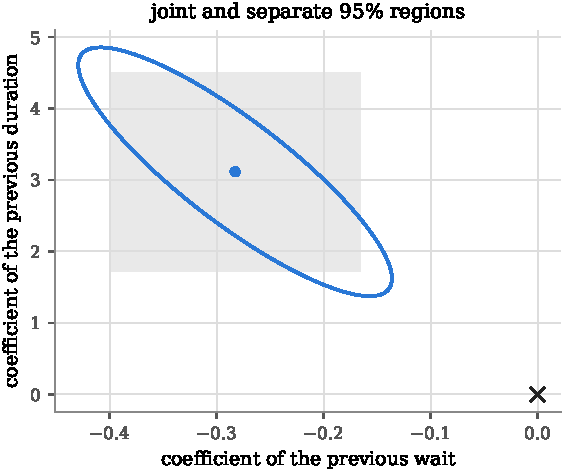
\includegraphics[width=0.52\textwidth]{fig_mreg_ellipse}
\caption{Old Faithful, the model with the duration, the previous wait and the previous duration: the joint $95\%$ confidence ellipse for the last two coefficients (blue), the two separate $95\%$ intervals (gray rectangle), the estimates (dot) and the origin (cross).}
\label{fig:mregellipse}
\end{figure}

\Cref{fig:mregellipse} draws the joint $95\%$ confidence region for the two coefficients in the full model, the ellipse $\{b : (\hat{b} - b)^\top C^{-1}(\hat{b} - b) \leq 2q_{0.05}(F_{2, 267})\}$ with $C$ the $2 \times 2$ block of $\hat{\sigma}^2(X^\top X)^{-1}$ (\cref{ex:mreg-ellipse}), together with the two separate intervals.
The ellipse is long and tilted, from upper left to lower right. Raise the previous wait's coefficient by $t$, lower the previous duration's by $11t$ and the intercept by $33t$, and the fitted values barely move, since the previous wait is close to $33 + 11 \times$ the previous duration, so the three columns nearly cancel in that combination; the data leave it loose, and it is the long axis of the ellipse. The combination along the short axis, $11$ times the previous wait's coefficient plus the previous duration's, is pinned down far better than either coefficient alone: its standard error is $0.37$, against $0.71$ for the previous duration's coefficient.
It is a mild form of the collinearity pitfall.
The origin lies far outside the ellipse, so the pair is clearly needed, and \cref{sec:mreg-ftest} gives the test that says so in one number.

\begin{pitfall}[what a coefficient does not say]
$\beta_j$ is the change in $\E[Y]$ per unit of predictor $j$ with the others held fixed, in a model containing exactly those others. It is not the effect of changing predictor $j$: the stack loss plant was observed, not manipulated, and the days with high air flow may have differed in ways the three columns do not record. A regression shows how the response moves with the predictors in the data; an experiment that sets the predictors, as the Physicians' Health Study of \cref{ex:reg-aspirin} assigned aspirin by randomization, is what shows what changing them does.
\end{pitfall}

\section{Several coefficients at once: the \texorpdfstring{$F$}{F}-test}
\label{sec:mreg-ftest}

`Does the acid concentration matter?' is one coefficient; `do the water temperature and the acid concentration matter, given the air flow?' is two.
Testing them one at a time at level $\alpha$ each does not give a test of level $\alpha$ for the pair, as \cref{ch:t-test} explained for many tests at once, and the previous worked example shows the stakes: there, both single tests failed and the pair was decisive.
The right test compares the fit with the predictors in question to the fit without them.

Let $X_0$ consist of the first $p - k$ columns of $X$, the predictors not under test, and let $\norm{e_0}^2$ be the residual sum of squares of the least squares fit with $X_0$ alone; it is at least $\norm{e}^2$, since the smaller model is a special case of the larger.

\begin{theorem}[The $F$-test]
\label{thm:mreg-ftest}
In the Gaussian linear model with $X$ of rank $p$, test $H_0: \beta_{p-k+1} = \cdots = \beta_p = 0$ against the alternative that at least one of them is not $0$.
Under $H_0$,
\[
F = \frac{(\norm{e_0}^2 - \norm{e}^2)/k}{\norm{e}^2/(n - p)} \sim F_{k, n-p},
\]
the $F$ distribution of \cref{ch:t-test}, so the test that rejects when $F > q_\alpha(F_{k, n-p})$ has level exactly $\alpha$.
It is the likelihood ratio test of \cref{ch:wald-lrt}: $T^{\mathrm{LR}}_n = n\log(\norm{e_0}^2/\norm{e}^2)$, an increasing function of $F$.
For $k = 1$, $F = T_p^2$, and the $F$-test is the two-sided $t$-test.
\end{theorem}
\coreproof{Split the error vector along three orthogonal subspaces: the column space of $X_0$, the part of the column space of $X$ perpendicular to it ($k$ dimensions), and the residual space ($n - p$ dimensions). Under $H_0$ the numerator is the squared length of the middle piece and the denominator that of the last; Cochran makes them independent chi-squareds.}
\begin{proof}
Let $P_0$ be the projection onto the column space of $X_0$ and $P$ onto that of $X$; the first space is inside the second, so $PP_0 = P_0$ and $P - P_0$ is the projection onto the part of the column space of $X$ perpendicular to the column space of $X_0$, a subspace of dimension $p - (p - k) = k$ \toolkit{sec:math-matrices}.
Then $e_0 = (I - P_0)Y$, $e = (I - P)Y$, and since $(I - P_0) = (P - P_0) + (I - P)$ with the two pieces perpendicular, Pythagoras gives
\[
\norm{e_0}^2 - \norm{e}^2 = \norm{(P - P_0)Y}^2.
\]
Under $H_0$, $X\beta = X_0\beta_0$ lies in the column space of $X_0$, so $(P - P_0)X\beta = 0$ and $(I - P)X\beta = 0$: both pieces are the same projections of $\epsilon$ alone.
Choose the orthonormal basis of the proof of \cref{thm:mreg-exact} so that $u_1, \ldots, u_{p-k}$ span the column space of $X_0$ and $u_1, \ldots, u_p$ that of $X$ (Gram--Schmidt applied to the columns of $X_0$ first, then the rest).
With $Z = Q\epsilon$ as before, $\norm{(P - P_0)\epsilon}^2 = Z_{p-k+1}^2 + \cdots + Z_p^2$ and $\norm{(I - P)\epsilon}^2 = Z_{p+1}^2 + \cdots + Z_n^2$: by \cref{prop:cochran-general} with the three subspaces, these are $\sigma^2$ times independent $\chi^2_k$ and $\chi^2_{n-p}$ variables, and the ratio of each to its degrees of freedom is $F_{k, n-p}$ by \cref{ch:t-test}'s definition.

For the likelihood ratio, the maximized log-likelihood of a Gaussian linear model is, by (3) of \cref{thm:mreg-exact}, $-\frac{n}{2}\log(2\pi\hat{\sigma}^2_{\mathrm{MLE}}) - \frac{n}{2}$ with $\hat{\sigma}^2_{\mathrm{MLE}} = \norm{e}^2/n$; the difference of the two models' maxima, times $2$, is $n\log(\norm{e_0}^2/\norm{e}^2) = n\log(1 + kF/(n - p))$, increasing in $F$.
For $k = 1$ the $k$-dimensional piece is one coordinate, $Z_p = u_p^\top\epsilon$, and under $H_0$, $\hat{\beta}_p = \sqrt{\gamma_p}\,Z_p$ (\cref{ex:mreg-t-f}), so $F = Z_p^2/\hat{\sigma}^2 = \hat{\beta}_p^2/(\gamma_p\hat{\sigma}^2) = T_p^2$; \cref{ex:mreg-t-f} shows that $F = T_p^2$ holds whether or not $H_0$ is true.
\end{proof}

\begin{worked}[two $F$-tests for the stack loss]
Do the three predictors together do anything? With $X_0$ the column of ones, $\norm{e_0}^2 = 2{,}069.2$, so
\[
F = \frac{(2{,}069.2 - 178.8)/3}{178.8/17} = \frac{630.1}{10.52} = 59.9
\]
on $(3, 17)$ degrees of freedom, against $q_{0.05}(F_{3, 17}) = 3.20$: $p$-value $3 \times 10^{-9}$. Do the water temperature and the acid add anything to the air flow? The fit on the air flow alone has $\norm{e_0}^2 = 319.1$, so $F = (319.1 - 178.8)/2 \div 10.52 = 70.2/10.52 = 6.67$ on $(2, 17)$ against $3.59$: $p$-value $0.007$, so of $1{,}000$ plants on which the water and the acid did nothing, about $7$ would give an $F$ this large. For Old Faithful, adding the previous wait and the previous duration to the duration gives $F = 11.5$ on $(2, 267)$, $p$-value $2 \times 10^{-5}$, where the two single $t$-tests found nothing.
\end{worked}

Any $k$ independent linear constraints on $\beta$, such as $\beta_2 = \beta_3$, take this form after a change of columns (with columns $x_2 + x_3$ and $x_3$ in place of $x_2$ and $x_3$, the coefficients are $\beta_2$ and $\beta_3 - \beta_2$), so the $F$-test covers the implicit hypotheses of \cref{ch:wald-lrt} as well.
Wilks' theorem (\cref{ch:wald-lrt}) would make $T^{\mathrm{LR}}_n$ approximately $\chi^2_k$; here Cochran's theorem makes $F$ exactly $F_{k, n-p}$, and as $n \to \infty$ with $k$ fixed, $kF \convd \chi^2_k$ (\cref{ex:mreg-f-chisq}), so the two agree in the limit.

\begin{bridge}[the ANOVA table and $R^2$]
Regression output's analysis-of-variance table is the first $F$-test above: the regression sum of squares $\norm{e_0}^2 - \norm{e}^2 = \sum_i (\hat{Y}_i - \bar{Y})^2$ on $p - 1$ degrees of freedom, the residual sum of squares on $n - p$, their mean squares, and their ratio $F$. Its $R^2 = 1 - \norm{e}^2/\norm{e_0}^2$ is the share of $\sum_i (Y_i - \bar{Y})^2$ that the fit accounts for ($0.914$ for the stack loss), and $F = \frac{R^2/(p - 1)}{(1 - R^2)/(n - p)}$ is the same number read off $R^2$. Adding a column never lowers $R^2$, since the larger model contains the smaller, which is why a high $R^2$ with many predictors proves little and the $F$-test, which charges each added column its degree of freedom, is the honest comparison.
\end{bridge}

\begin{remark}[Bonferroni's test]
An alternative to the $F$-test rejects $H_0$ when any one of the $k$ single tests rejects at level $\alpha/k$: by the union bound of \cref{prop:bonferroni}, its level is at most $\alpha$. For the water temperature and the acid, $\alpha/2 = 0.025$ gives the threshold $q_{0.0125}(t_{17}) = 2.458$, and $T = 3.52$ for the water rejects. Bonferroni does not need the $k$ tests to come from one model or one data set, and when it rejects it says which hypothesis failed, which the $F$-test does not; its price is the conservative level, and a case like Old Faithful's two predictors, where each single $T$ is small in its own smaller model, is exactly where it can miss what the $F$-test sees.
\end{remark}

\section{Ridge in matrix form}
\label{sec:mreg-ridge}

\Cref{ch:regression-uni} shrank one slope toward $0$ by adding a Gaussian prior; with $p$ coefficients the same prior on each gives the matrix form.
Under the Gaussian linear model with $\sigma^2$ known and the prior $\beta \sim \Gauss_p(0, \tau^2 I_p)$, the log posterior density is, up to a constant,
\[
-\frac{1}{2\sigma^2}\norm{Y - X\beta}^2 - \frac{1}{2\tau^2}\norm{\beta}^2,
\]
whose gradient in $\beta$ \toolkit{sec:math-multivar} is $\sigma^{-2}(X^\top Y - X^\top X\beta) - \tau^{-2}\beta$, zero at the \textbf{ridge estimator}
\[
\tilde{\beta}_\lambda = (X^\top X + \lambda I_p)^{-1}X^\top Y, \qquad \lambda = \frac{\sigma^2}{\tau^2},
\]
which minimizes $\norm{Y - X\beta}^2 + \lambda\norm{\beta}^2$.

\begin{figure}[htbp]
\centering
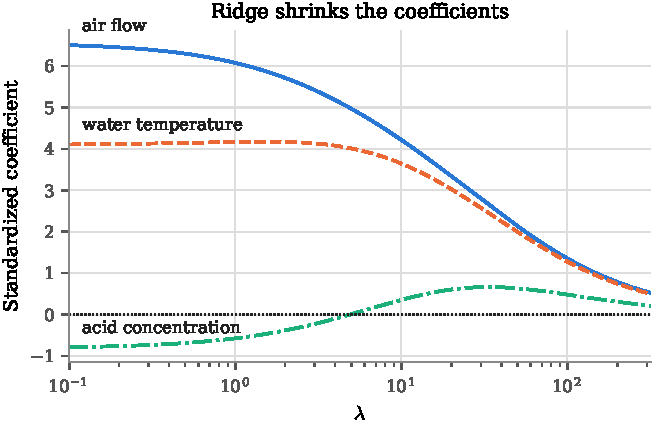
\includegraphics[width=0.72\textwidth]{fig_mreg_ridge}
\caption{Ridge on the stack loss data with standardized predictors: the coefficients of the air flow (blue), the water temperature (orange, dashed) and the acid concentration (aqua, dash-dot) against $\lambda$ on a logarithmic axis.}
\label{fig:mregridge}
\end{figure}

Since $a^\top(X^\top X + \lambda I)a = \norm{Xa}^2 + \lambda\norm{a}^2 > 0$ for $a \neq 0$ and $\lambda > 0$, the matrix is invertible whatever the rank of $X$: ridge has a unique answer even for collinear columns, where least squares has infinitely many, and a steady one when they are nearly collinear.
In practice the intercept is left out of the penalty and the predictors are standardized first, so that one $\lambda$ treats them alike.
\Cref{fig:mregridge} does this for the stack loss data: as $\lambda$ grows the three standardized coefficients leave their least squares values $(6.56, 4.09, -0.82)$, the air flow's and the water temperature's shrinking toward $0$ and the acid's, whose sign is not even determined by the data, crossing $0$ near $\lambda = 5$ before it too heads to $0$.
Choosing $\lambda$ is choosing $\tau$, the prior spread of the coefficients, and \cref{ex:reg-ridge} showed why a small positive $\lambda$ lowers the risk whatever $\beta$ is.

\section{Without Gaussian errors, and checking the model}
\label{sec:mreg-robust}

Nothing in parts (1) and (2) of \cref{thm:mreg-exact} needed Gaussian errors, and the large-sample theory of \cref{thm:lse-asymptotic} extends to $p$ predictors by the same route, with vectors in place of numbers.

\begin{theorem}[Least squares with $p$ predictors, without Gaussian errors]
\label{thm:mreg-asymptotic}
Let $(x_1, Y_1), (x_2, Y_2), \ldots$ be i.i.d.\ copies of $(x, Y) \in \real^p \times \real$ with finite fourth moments, let $M = \E[xx^\top]$ be positive definite, let $\beta^*$ minimize $\E[(Y - x^\top\beta)^2]$ and $\epsilon = Y - x^\top\beta^*$, and let $V = \E[\epsilon^2xx^\top]$ be positive definite.
Then $\hat{\beta} \convp \beta^*$ and
\[
\sqrt{n}(\hat{\beta} - \beta^*) \convd \Gauss_p(0, M^{-1}VM^{-1}).
\]
If $\E[\epsilon^2 \mid x] = \sigma^2$, then $M^{-1}VM^{-1} = \sigma^2M^{-1}$, $\hat{\sigma}^2 \convp \sigma^2$, and each $T_j$ of \cref{sec:mreg-ttest} converges in distribution to $\Gauss(0, 1)$ under $\beta_j^* = 0$.
\end{theorem}
\optionalproof{The one-predictor proof with matrices: $\hat{\beta} - \beta^* = (\frac1n X^\top X)^{-1}\frac1n X^\top\epsilon$, the Law of Large Numbers for the first factor and the vector Central Limit Theorem for the second.}
\recall{The Law of Large Numbers (\cref{thm:wlln}) for each entry of an average of i.i.d.\ matrices with finite variances; the continuous mapping theorem (\cref{thm:cmt}) for the inverse, continuous at an invertible matrix; the Central Limit Theorem for vectors (the vector-versions remark of \cref{ch:limit-tools}): for i.i.d.\ vectors $W_i$ with mean $0$ and positive definite covariance $V$, $\sqrt{n}\,\bar{W}_n \convd \Gauss_p(0, V)$; Slutsky's theorem (\cref{thm:slutsky}), as \cref{ch:wald-lrt} uses it for vectors: if $A_n \convp A$, a fixed matrix, and $W_n \convd W$, then $(A_n - A)W_n \convp 0$ entry by entry and $A_nW_n \convd AW$.}
\begin{proof}
The minimizer $\beta^*$ solves $\E[x(Y - x^\top\beta)] = 0$, since the gradient of $\E[(Y - x^\top\beta)^2]$ is $-2\E[x(Y - x^\top\beta)] = -2(\E[xY] - M\beta)$, so $\beta^* = M^{-1}\E[xY]$ and $\E[x\epsilon] = 0$.
Writing $Y_i = x_i^\top\beta^* + \epsilon_i$ in the formula for $\hat{\beta}$,
\[
\hat{\beta} - \beta^* = \Big(\frac1n\sum_i x_ix_i^\top\Big)^{-1}\frac1n\sum_i x_i\epsilon_i.
\]
By the Law of Large Numbers, entry by entry, $\frac1n\sum_i x_ix_i^\top \convp M$ (finite fourth moments make the variances finite), so $X^\top X$ is invertible, and $\hat{\beta}$ defined, with probability tending to $1$; the inverse is continuous at $M$, so the first factor converges in probability to $M^{-1}$. The second is an average of i.i.d.\ vectors $W_i = x_i\epsilon_i$ with mean $0$ and covariance $V$, which is finite since $\epsilon$, a linear combination of $Y$ and the entries of $x$, has a finite fourth moment and $\epsilon^2\abs{x_jx_k} \leq \frac12(\epsilon^4 + x_j^2x_k^2)$; so it converges in probability to $0$, and $\sqrt{n}$ times it converges in distribution to $\Gauss_p(0, V)$.
Slutsky's theorem gives $\hat{\beta} \convp \beta^*$ and $\sqrt{n}(\hat{\beta} - \beta^*) \convd M^{-1}\Gauss_p(0, V) = \Gauss_p(0, M^{-1}VM^{-1})$, by the linear-map rule for Gaussian vectors \toolkit{sec:math-gaussquad}.
If $\E[\epsilon^2 \mid x] = \sigma^2$, then $V = \E[xx^\top\E[\epsilon^2 \mid x]] = \sigma^2M$ by taking out what is known and the tower property \toolkit{sec:math-condexp}, and $M^{-1}VM^{-1} = \sigma^2M^{-1}$.
For $\hat{\sigma}^2$, $e = \epsilon - X(\hat{\beta} - \beta^*)$ and $X^\top e = 0$ give $\norm{e}^2 = \norm{\epsilon}^2 - \norm{X(\hat{\beta} - \beta^*)}^2$, and $\frac1n\norm{X(\hat{\beta} - \beta^*)}^2 = (\hat{\beta} - \beta^*)^\top\frac1n X^\top X(\hat{\beta} - \beta^*) \convp 0$, so $\hat{\sigma}^2 = \frac{n}{n-p}\cdot\frac1n\norm{e}^2 \convp \E[\epsilon^2] = \sigma^2$, by the Law of Large Numbers for the $\epsilon_i^2$, whose variance is finite by the fourth moments.
Then $T_j = \sqrt{n}\hat{\beta}_j\big/\big(\hat{\sigma}\sqrt{n\gamma_j}\big)$, where $n\gamma_j$, the $j$th diagonal entry of $(\frac1n X^\top X)^{-1}$, converges in probability to that of $M^{-1}$, and Slutsky's theorem finishes it.
\end{proof}

So the $t$-tests and intervals keep their level for large $n$ whatever the errors' distribution, as long as the scatter is the same everywhere; when it is not, the sandwich $M^{-1}VM^{-1}$, estimated by plugging in $\frac1n\sum_i x_ix_i^\top$ and $\frac1n\sum_i e_i^2x_ix_i^\top$, gives the robust standard errors of \cref{ch:mom-mestimation}'s bridge, the $p$-predictor form of the one in \cref{ch:regression-uni}; as there, the consistency of the plug-in estimate is stated and not proved.
The $F$-test survives the same way: $kF \convd \chi^2_k$ under $H_0$ for constant scatter (\cref{ex:mreg-f-chisq}).

What the theory cannot do is tell you whether the model is any good, and the residuals are the place to look.
In the Gaussian linear model the residuals are the projection $(I - P)\epsilon$ of the errors, so they should look like mean-zero noise with no pattern against the fitted values or against any predictor: a curve in such a plot says that the mean is not linear, a fan says that the scatter changes with the mean.
The right of \cref{fig:mregstackloss} shows neither for the stack loss, apart from day $21$.
Whether the errors are Gaussian can be tested with the residuals in place of the errors: the Lilliefors test of \cref{ch:ks} on the $21$ stack loss residuals gives $D = 0.107$ against a $5\%$ threshold of $0.19$, no evidence against normality, with two caveats: the threshold is approximate, since the residuals are correlated and their variances differ (\cref{ex:mreg-projection}), and $n = 21$ has little power (\cref{sec:ks-lilliefors}).
For the exactness of the $t$- and $F$-tests at $n = 21$ that is what matters. At $n = 271$ Old Faithful's whole-minute waits are covered by \cref{thm:mreg-asymptotic}, but its rows are not independent, and in the model with the previous wait as a predictor they cannot be: the previous wait is the response of the row before. The $t$ and $F$ statistics for that model are the ones the Gaussian linear model prescribes, and large-sample theory for such lagged designs, which this book does not develop, supports them approximately, as the remarks of \cref{sec:reg-inference} did for consecutive eruptions.

\section{What comes next}
\label{sec:mreg-next}

This chapter closes Part VIII.
The response has been a number whose mean is linear in the predictors and whose scatter is the same everywhere.
For the kiss data's $0$s and $1$s, or for counts, neither holds: a mean that is a probability cannot be a line in the predictors without leaving $[0, 1]$, and the variance $p(1 - p)$ moves with the mean.
Part IX keeps the linear predictor $x^\top\beta$ and changes what it is linked to: \cref{ch:exp-families} describes the distributions for which this works, the exponential families, and \cref{ch:glm-links} links their means to $x^\top\beta$ through a function such as the log-odds of \cref{ch:jeffreys}, with maximum likelihood, now without a closed form, doing the fitting.

\section{Summary}
\label{sec:mreg-summary}

\begin{itemize}[nosep]
\item $Y = X\beta + \epsilon$ with an $n \times p$ design matrix, $\E[\epsilon] = 0$, $\cov(\epsilon) = \sigma^2I_n$; polynomials, $0/1$ variables and lagged values are columns like any other. Full rank of $X$ is identifiability; collinearity is its failure.
\item $\hat{\beta} = (X^\top X)^{-1}X^\top Y$ is unique when $X$ has rank $p$; $X\hat{\beta} = PY$ is the projection of $Y$ onto the column space, $e \perp$ every column (the normal equations $X^\top e = 0$). Stack loss: $-39.92 + 0.716\,\text{air} + 1.295\,\text{water} - 0.152\,\text{acid}$, $R^2 = 0.914$.
\item $\E[\hat{\beta}] = \beta$, $\cov(\hat{\beta}) = \sigma^2(X^\top X)^{-1}$, risk $\sigma^2\,\mathrm{tr}((X^\top X)^{-1})$; $\hat{\sigma}^2 = \norm{e}^2/(n - p)$ is unbiased. Gaussian errors: $\hat{\beta} \sim \Gauss_p(\beta, \sigma^2(X^\top X)^{-1})$ is the MLE, $(n - p)\hat{\sigma}^2/\sigma^2 \sim \chi^2_{n-p}$ independent of $\hat{\beta}$ (Cochran, general form), $(\hat{\beta}_j - \beta_j)/(\hat{\sigma}\sqrt{\gamma_j}) \sim t_{n-p}$.
\item One coefficient: $T_j = \hat{\beta}_j/(\hat{\sigma}\sqrt{\gamma_j})$ against $q_{\alpha/2}(t_{n-p})$; stack loss $T = 5.31, 3.52, -0.97$. A coefficient is a statement about a model: the air flow's $1.02$ alone, $0.72$ with the others; Old Faithful's previous wait and previous duration, useless alone and decisive together.
\item Several coefficients: $F = \frac{(\norm{e_0}^2 - \norm{e}^2)/k}{\norm{e}^2/(n - p)} \sim F_{k, n-p}$ under $H_0$, the likelihood ratio test made exact; $F = T^2$ for $k = 1$; stack loss $59.9$ on $(3, 17)$ and $6.67$ on $(2, 17)$; Old Faithful $11.5$ on $(2, 267)$. Bonferroni, $\alpha/k$ per test, has level at most $\alpha$ and says which hypothesis failed.
\item Ridge: $(X^\top X + \lambda I)^{-1}X^\top Y$, the posterior mode under $\beta \sim \Gauss_p(0, \tau^2I)$, $\lambda = \sigma^2/\tau^2$; defined for every $X$.
\item Without Gaussian errors, for i.i.d.\ rows: $\sqrt{n}(\hat{\beta} - \beta^*) \convd \Gauss_p(0, M^{-1}VM^{-1})$, which is $\sigma^2M^{-1}$ for constant scatter; the sandwich otherwise. Check the residuals against the fitted values, and their normality with Lilliefors.
\end{itemize}

\section{Exercises}
\label{sec:mreg-exercises}

\begin{exercise}
\label{ex:mreg-onepred}
Take $X$ with columns $(1, \ldots, 1)^\top$ and $(x_1, \ldots, x_n)^\top$. (a) Compute $X^\top X$, $X^\top Y$ and $(X^\top X)^{-1}$, and show that $\hat{\beta} = (X^\top X)^{-1}X^\top Y$ is the pair $(\hat{a}, \hat{b})$ of \cref{thm:lse}. (b) Show that $\sigma^2(X^\top X)^{-1}$ is the covariance matrix of \cref{prop:lse-moments}.
\end{exercise}
\begin{solution}
(a) $X^\top X = \begin{pmatrix} n & \sum_i x_i \\ \sum_i x_i & \sum_i x_i^2\end{pmatrix}$, $X^\top Y = (\sum_i Y_i, \sum_i x_iY_i)^\top$, and $\det(X^\top X) = n\sum_i x_i^2 - (\sum_i x_i)^2 = nS_{xx}$, so $(X^\top X)^{-1} = \frac{1}{nS_{xx}}\begin{pmatrix} \sum_i x_i^2 & -n\bar{x} \\ -n\bar{x} & n\end{pmatrix}$. The second row gives
\[
\hat{b} = \frac{n\sum_i x_iY_i - n\bar{x}\sum_i Y_i}{nS_{xx}} = \frac{S_{xy}}{S_{xx}}, \qquad \hat{a} = \frac{\sum_i x_i^2\sum_i Y_i - n\bar{x}\sum_i x_iY_i}{nS_{xx}} = \bar{Y} - \hat{b}\bar{x},
\]
the second after writing $\sum_i x_i^2 = S_{xx} + n\bar{x}^2$. (b) $\sigma^2$ times the entries: $\var(\hat{b}) = \sigma^2/S_{xx}$, $\var(\hat{a}) = \sigma^2\sum_i x_i^2/(nS_{xx}) = \sigma^2(1/n + \bar{x}^2/S_{xx})$, $\cov(\hat{a}, \hat{b}) = -\sigma^2\bar{x}/S_{xx}$.
\end{solution}

\begin{exercise}
\label{ex:mreg-groups}
Two groups. Let $X$ have a column of ones and a column $z$ of $0$s and $1$s, with $n_1$ ones and $n_0 = n - n_1$ zeros. (a) Compute $(X^\top X)^{-1}$ and show that $\hat{\beta} = (\bar{Y}_0, \bar{Y}_1 - \bar{Y}_0)^\top$. (b) Show that $\gamma_2 = 1/n_0 + 1/n_1$, so that $T_2$ is the pooled two-sample $t$ statistic of \cref{thm:pooled-t} and the $t$-test for $\beta_2 = 0$ is the pooled $t$-test. (c) In the aspirin study, $n_0 = 11{,}034$ and $n_1 = 11{,}037$; verify $\gamma_2$ and the standard error $0.00154$ of \cref{ex:reg-aspirin}.
\end{exercise}
\begin{solution}
(a) $X^\top X = \begin{pmatrix} n & n_1 \\ n_1 & n_1\end{pmatrix}$, with inverse $\frac{1}{nn_1 - n_1^2}\begin{pmatrix} n_1 & -n_1 \\ -n_1 & n\end{pmatrix} = \frac{1}{n_0}\begin{pmatrix} 1 & -1 \\ -1 & n/n_1\end{pmatrix}$, and $X^\top Y = (n_0\bar{Y}_0 + n_1\bar{Y}_1, n_1\bar{Y}_1)^\top$, giving $\hat{\beta}_1 = \bar{Y}_0$ and $\hat{\beta}_2 = \bar{Y}_1 - \bar{Y}_0$. (b) $\gamma_2 = n/(n_0n_1) = 1/n_0 + 1/n_1$, and $\hat{\sigma}^2$ is the pooled variance (the residuals are the deviations within each group, on $n - 2$ degrees of freedom), so $T_2 = (\bar{Y}_1 - \bar{Y}_0)/(\hat{\sigma}\sqrt{1/n_0 + 1/n_1})$. (c) $\gamma_2 = 1/11{,}034 + 1/11{,}037 = 1.8124 \times 10^{-4}$, and with $\hat{\sigma}^2 = 0.01309$ the standard error is $\sqrt{0.01309 \times 1.8124 \times 10^{-4}} = 0.00154$.
\end{solution}

\begin{exercise}
\label{ex:mreg-projection}
Let $P = X(X^\top X)^{-1}X^\top$ with $X$ of rank $p$. (a) Show that $\mathrm{tr}(P) = p$ and $\mathrm{tr}(I - P) = n - p$, using $\mathrm{tr}(AB) = \mathrm{tr}(BA)$. (b) Deduce $\E\norm{e}^2 = (n - p)\sigma^2$ directly from $e = (I - P)\epsilon$ and $\E[\epsilon\epsilon^\top] = \sigma^2I$, without the rotation. (c) The diagonal entry $P_{ii}$ is called the leverage of observation $i$; show that $\var(e_i) = \sigma^2(1 - P_{ii})$, so a high-leverage observation has a small residual however badly it fits. For the stack loss data the largest leverage is $0.41$, on day $17$, and $\mathrm{tr}(P) = 4$.
\end{exercise}
\begin{solution}
(a) $\mathrm{tr}(P) = \mathrm{tr}\big((X^\top X)^{-1}X^\top X\big) = \mathrm{tr}(I_p) = p$, and $\mathrm{tr}(I_n - P) = n - p$. (b) $\norm{e}^2 = \epsilon^\top(I - P)^\top(I - P)\epsilon = \epsilon^\top(I - P)\epsilon = \mathrm{tr}\big((I - P)\epsilon\epsilon^\top\big)$, whose expectation is $\mathrm{tr}\big((I - P)\sigma^2I\big) = (n - p)\sigma^2$. (c) $\cov(e) = (I - P)\sigma^2I(I - P)^\top = \sigma^2(I - P)$, so $\var(e_i) = \sigma^2(1 - P_{ii})$; as $P_{ii} \to 1$ the residual's variance vanishes, so the fit passes near the observation whatever its value.
\end{solution}

\begin{exercise}
\label{ex:mreg-t-f}
For $k = 1$ in \cref{thm:mreg-ftest}, show that $\norm{e_0}^2 - \norm{e}^2 = \hat{\beta}_p^2/\gamma_p$, so that $F = T_p^2$. (Write $u_p$, the last basis vector of the proof, as $(I - P_0)x_p/\norm{(I - P_0)x_p}$ with $x_p$ the last column of $X$, and use $\hat{\beta}_p = u_p^\top Y/\norm{(I - P_0)x_p}$ and $\gamma_p = 1/\norm{(I - P_0)x_p}^2$; the last two follow from writing the fit of the full model as the fit of $X_0$ plus the fit of the residual of $x_p$ on $X_0$.)
\end{exercise}
\begin{solution}
Let $w = (I - P_0)x_p$, the part of the last column perpendicular to the column space of $X_0$; $w \neq 0$ since $X$ has full rank, and the column space of $X$ is spanned by the columns of $X_0$ together with $w$, with $w$ perpendicular to the first. So $P = P_0 + ww^\top/\norm{w}^2$ and $(P - P_0)Y = (w^\top Y/\norm{w}^2)w$, whose squared length is $(w^\top Y)^2/\norm{w}^2$. The coefficient of $x_p$ in the full fit is the coefficient of $w$ in $PY$, since replacing $x_p$ by $w$ only reparameterizes the $X_0$ coefficients: $\hat{\beta}_p = w^\top Y/\norm{w}^2$, and its variance $\sigma^2\gamma_p$ is $\sigma^2\norm{w}^2/\norm{w}^4 = \sigma^2/\norm{w}^2$. Hence $\norm{e_0}^2 - \norm{e}^2 = \hat{\beta}_p^2\norm{w}^2 = \hat{\beta}_p^2/\gamma_p$ and $F = \hat{\beta}_p^2/(\hat{\sigma}^2\gamma_p) = T_p^2$. For the stack loss acid coefficient, $(188.8 - 178.8)/10.52 = 0.95 = (-0.973)^2$.
\end{solution}

\begin{exercise}
\label{ex:mreg-f-chisq}
(a) Show that if $V \sim \chi^2_k$ and $W_n \sim \chi^2_{n-p}$ are independent, then $k\,\frac{V/k}{W_n/(n - p)} \convd \chi^2_k$ as $n \to \infty$ with $k$ and $p$ fixed. (b) Explain why, under the hypotheses of \cref{thm:mreg-asymptotic} with constant scatter and $H_0$ true, $kF \convd \chi^2_k$ even without Gaussian errors. (Write $\norm{e_0}^2 - \norm{e}^2$ as a quadratic form in $\sqrt{n}(\hat{\beta} - \beta^*)$'s last $k$ coordinates.)
\end{exercise}
\begin{solution}
(a) $W_n/(n - p)$ is the mean of $n - p$ i.i.d.\ $\chi^2_1$ variables, which converges in probability to $1$ by the Law of Large Numbers, so $kF = V/(W_n/(n - p)) \convd V$ by Slutsky's theorem. (b) Let $X_1$ be the last $k$ columns of $X$, $\hat{\beta}_{(k)}$ their coefficients and $C_{(k)}$ the matching block of $(X^\top X)^{-1}$, and let $W = (I - P_0)X_1$, the parts of those columns perpendicular to the column space of $X_0$; $W$ has rank $k$ since $X$ has rank $p$, and $X_1 = X_0A + W$ for some matrix $A$. As in the previous exercise the column space of $X$ is that of $X_0$ plus that of $W$, perpendicular to each other, so $P = P_0 + W(W^\top W)^{-1}W^\top$; and $X\beta = X_0(\beta_0 + A\beta_{(k)}) + W\beta_{(k)}$ shows that $\hat{\beta}_{(k)} = (W^\top W)^{-1}W^\top Y$, with covariance $\sigma^2(W^\top W)^{-1}$, so $C_{(k)} = (W^\top W)^{-1}$. Hence $\norm{e_0}^2 - \norm{e}^2 = \norm{(P - P_0)Y}^2 = Y^\top W(W^\top W)^{-1}W^\top Y = \hat{\beta}_{(k)}^\top C_{(k)}^{-1}\hat{\beta}_{(k)}$. Under $H_0$, $\sqrt{n}\hat{\beta}_{(k)} \convd \Gauss_k(0, \sigma^2 M^{-1}_{(k)})$ and $nC_{(k)} \convp M^{-1}_{(k)}$ by \cref{thm:mreg-asymptotic}, so the quadratic form converges in distribution to $\sigma^2\chi^2_k$ by \cref{lem:gauss-quadform} and the continuous mapping theorem; dividing by $\hat{\sigma}^2 \convp \sigma^2$ gives $kF \convd \chi^2_k$.
\end{solution}

\begin{exercise}
\label{ex:mreg-ellipse}
Joint confidence region. In the Gaussian linear model let $\hat{\beta}_{(k)}$ and $C_{(k)}$ be as in the previous exercise, and let $\hat{C}_{(k)} = \hat{\sigma}^2C_{(k)}$. Show that $(\hat{\beta}_{(k)} - \beta_{(k)})^\top\hat{C}_{(k)}^{-1}(\hat{\beta}_{(k)} - \beta_{(k)})/k \sim F_{k, n-p}$, so that the ellipsoid $\{b : (\hat{\beta}_{(k)} - b)^\top\hat{C}_{(k)}^{-1}(\hat{\beta}_{(k)} - b) \leq k\,q_\alpha(F_{k, n-p})\}$ is a confidence region of level $1 - \alpha$ for $\beta_{(k)}$. This is the ellipse of \cref{fig:mregellipse}, with $k = 2$ and $2q_{0.05}(F_{2, 267}) = 6.06$.
\end{exercise}
\begin{solution}
$\hat{\beta}_{(k)} \sim \Gauss_k(\beta_{(k)}, \sigma^2C_{(k)})$ by the linear-map rule, so by \cref{lem:gauss-quadform} the quadratic form $(\hat{\beta}_{(k)} - \beta_{(k)})^\top(\sigma^2C_{(k)})^{-1}(\hat{\beta}_{(k)} - \beta_{(k)})$ is $\chi^2_k$, independent of $(n - p)\hat{\sigma}^2/\sigma^2 \sim \chi^2_{n-p}$ by \cref{thm:mreg-exact}. Replacing $\sigma^2$ by $\hat{\sigma}^2$ multiplies the quadratic form by $\sigma^2/\hat{\sigma}^2$, so the quantity in the exercise is $(\chi^2_k/k)/(\chi^2_{n-p}/(n - p))$ with independent numerator and denominator: $F_{k, n-p}$. The ellipsoid contains $\beta_{(k)}$ exactly when this statistic is at most $q_\alpha(F_{k, n-p})$, which has probability $1 - \alpha$.
\end{solution}

\begin{exercise}
\label{ex:mreg-quadratic}
Polynomial regression. For Old Faithful, fitting the waits on $1$, $x$ and $x^2$ gives $\hat{\beta} = (17.20, 22.21, -1.766)^\top$ with $T = -3.74$ for the squared term and residual sum of squares $8{,}976.7$, against $9{,}443.4$ for the line. (a) Compute the $F$ statistic for the squared term and check that it equals $T^2$. (b) The fitted parabola's slope at $x$ is $22.21 - 3.53x$; evaluate it at $2$ and at $4.5$ minutes and relate the numbers to the residual plot of \cref{fig:reglsfit}. (c) Why is this still a linear regression?
\end{exercise}
\begin{solution}
(a) $F = (9{,}443.4 - 8{,}976.7)/1 \div 8{,}976.7/269 = 466.7/33.37 = 13.99 = (-3.74)^2$. (b) $15.1$ minutes per minute at $2$ minutes and $6.3$ at $4.5$: the waits rise faster than the line for short eruptions and more slowly for long ones, which is the bend in the bin means of \cref{fig:reglsfit}. (c) The model is linear in the coefficients: $x^2$ is a column of numbers computed from the durations, and $Y = X\beta + \epsilon$ with that column is \cref{def:mreg-model}.
\end{solution}

\begin{exercise}
\label{ex:mreg-gm}
Gauss--Markov in general. In the linear regression model with $X$ of rank $p$, let $\tilde{\beta} = AY$ be any estimator that is linear in $Y$ and unbiased for every $\beta$. (a) Show that $AX = I_p$. (b) Write $A = (X^\top X)^{-1}X^\top + D$ and show that $DX = 0$. (c) Show that $\cov(\tilde{\beta}) = \sigma^2(X^\top X)^{-1} + \sigma^2DD^\top$, so that every coordinate of $\hat{\beta}$ has the smallest variance among linear unbiased estimators.
\end{exercise}
\begin{solution}
(a) $\E[AY] = AX\beta$ equals $\beta$ for every $\beta$ only if $AX = I_p$. (b) $DX = AX - (X^\top X)^{-1}X^\top X = I_p - I_p = 0$. (c) $\cov(AY) = \sigma^2AA^\top$, and $AA^\top = (X^\top X)^{-1}X^\top X(X^\top X)^{-1} + (X^\top X)^{-1}X^\top D^\top + DX(X^\top X)^{-1} + DD^\top$; the two middle terms vanish since $DX = 0$ and $(DX)^\top = X^\top D^\top = 0$. The diagonal of $DD^\top$ is $\sum_k D_{jk}^2 \geq 0$, so $\var(\tilde{\beta}_j) \geq \var(\hat{\beta}_j)$ for each $j$; this is \cref{prop:gauss-markov} for every coordinate at once.
\end{solution}

\begin{exercise}
\label{ex:mreg-ridge-bias}
For the ridge estimator with $X$ of rank $p$, (a) show that $\E[\tilde{\beta}_\lambda] = (X^\top X + \lambda I)^{-1}X^\top X\beta$, so it is biased for $\lambda > 0$, and that $\cov(\tilde{\beta}_\lambda) = \sigma^2(X^\top X + \lambda I)^{-1}X^\top X(X^\top X + \lambda I)^{-1}$; (b) when $X^\top X = cI_p$ (orthogonal columns of equal length), show that $\tilde{\beta}_\lambda = \frac{c}{c + \lambda}\hat{\beta}$, the one-predictor shrinkage of \cref{sec:reg-gauss} applied to every coordinate.
\end{exercise}
\begin{solution}
(a) $\tilde{\beta}_\lambda = (X^\top X + \lambda I)^{-1}X^\top(X\beta + \epsilon)$; the expectation is the first term and the covariance is $(X^\top X + \lambda I)^{-1}X^\top\,\sigma^2I\,X(X^\top X + \lambda I)^{-1}$. (b) $(cI + \lambda I)^{-1}X^\top Y = \frac{1}{c + \lambda}X^\top Y$ and $\hat{\beta} = \frac1cX^\top Y$, so $\tilde{\beta}_\lambda = \frac{c}{c + \lambda}\hat{\beta}$, which is the factor $S_{xx}/(S_{xx} + \lambda)$ with $c$ in place of $S_{xx}$.
\end{solution}

\begin{exercise}
\label{ex:mreg-kiss}
The kiss data as a regression. (a) With $X$ the column of ones, compute $(X^\top X)^{-1}$, $\hat{\beta}$, $P$ and $\mathrm{tr}(P)$. (b) Suppose the $124$ couples had been observed in two cities, $60$ in the first with $36$ right turns and $64$ in the second with $44$, and add the city as a $0/1$ column. Compute $\hat{\beta}$, $\norm{e}^2$, $\hat{\sigma}^2$ and $T_2$, and say what the test of $\beta_2 = 0$ asks. (c) Which assumption of the Gaussian linear model fails, and what makes the test usable anyway?
\end{exercise}
\begin{solution}
(a) $X^\top X = 124$, $(X^\top X)^{-1} = 1/124$, $\hat{\beta} = \bar{R}_n = 0.645$, $P$ is the matrix with every entry $1/124$, whose trace is $1$. (b) By \cref{ex:mreg-groups}, $\hat{\beta} = (36/60, 44/64 - 36/60)^\top = (0.600, 0.0875)^\top$; $\norm{e}^2 = 36(0.4)^2 + 24(0.6)^2 + 44(0.3125)^2 + 20(0.6875)^2 = 5.76 + 8.64 + 4.30 + 9.45 = 28.15$, $\hat{\sigma}^2 = 28.15/122 = 0.2307$, $\gamma_2 = 1/60 + 1/64 = 0.03229$, and $T_2 = 0.0875/\sqrt{0.2307 \times 0.03229} = 1.01$: no evidence that the proportion turning right differs between the cities. (c) The errors take two values, so they are not Gaussian, and their variance $p(1 - p)$ differs slightly between the cities ($0.240$ and $0.215$). With the couples modeled as i.i.d.\ draws whose city is recorded, \cref{thm:mreg-asymptotic} applies without its constant-scatter condition, and the robust standard error, here the unpooled $\sqrt{0.240/60 + 0.215/64} = 0.0858$, makes the test asymptotically valid; it is within $1\%$ of the pooled $\hat{\sigma}\sqrt{\gamma_2} = 0.0863$, as in \cref{ex:reg-aspirin}.
\end{solution}
